\begin{figure}[!htb]
    \centering
    \begin{adjustbox}{minipage=\linewidth,scale=0.7}
    \Subfigure[0.8]{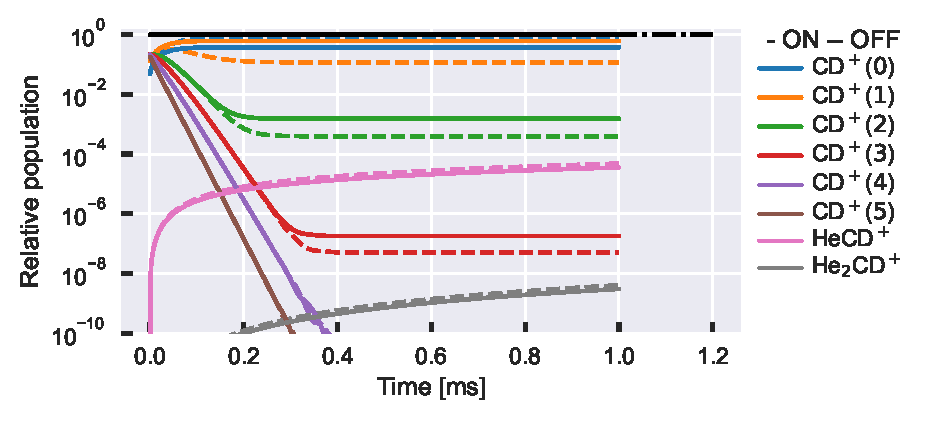
\includegraphics[width=1\textwidth]{figures/simulations/coll_rad_att/CD+_He_f-time__transition_0-1_0.001s_population_ratio.pdf}}{}{\label{fig:thz-sim:rel-pop:1ms}}
    \hfill
    
    \Subfigure[0.5]{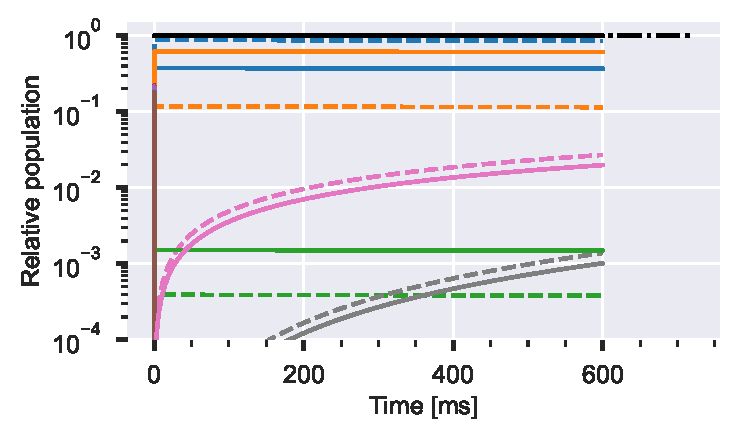
\includegraphics[width=1\textwidth]{figures/simulations/coll_rad_att/CD+_He_f-time__transition_0-1_0.6s_population_ratio.pdf}}{}{\label{fig:thz-sim:rel-pop:0.6s}}
    \hfill
    \Subfigure[0.45]{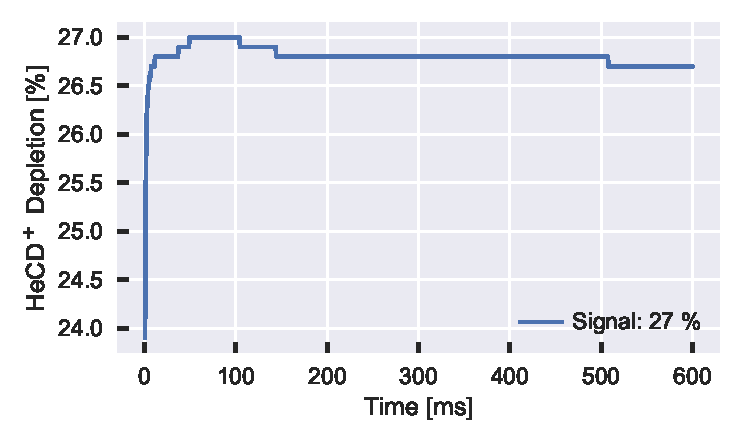
\includegraphics[width=1\textwidth]{figures/simulations/coll_rad_att/CD+_He_f-time__transition_0-1_0.6s_signal.pdf}}{}{\label{fig:thz-sim:signal:0.6s}}
    \hfill
    
    \Subfigure[0.5]{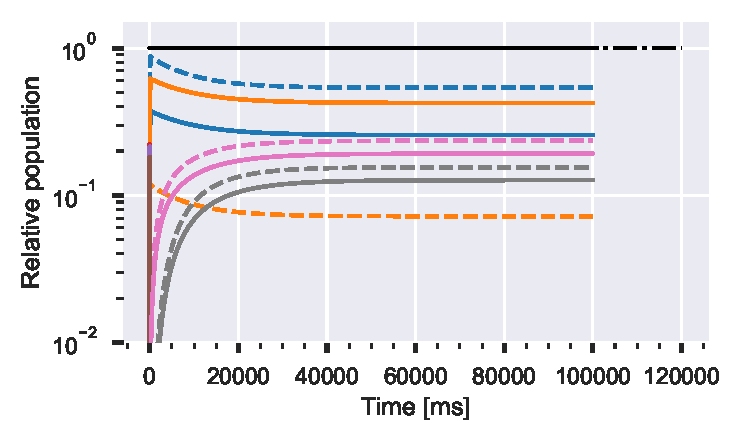
\includegraphics[width=1\textwidth]{figures/simulations/coll_rad_att/CD+_He_f-time__transition_0-1_100.0s_population_ratio.pdf}}{}{\label{fig:thz-sim:rel-pop:100s}}
    \hfill
    \Subfigure[0.45]{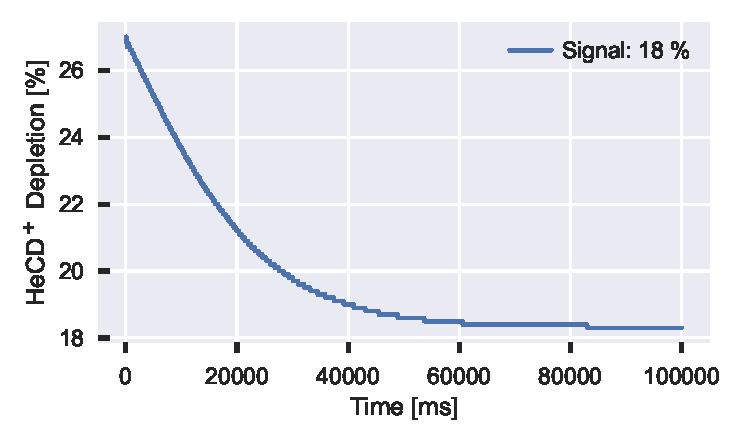
\includegraphics[width=1\textwidth]{figures/simulations/coll_rad_att/CD+_He_f-time__transition_0-1_100.0s_signal.pdf}}{}{\label{fig:thz-sim:signal:100s}}
    \hfill
    
    \end{adjustbox}
    
    \caption{
        (a) Simulated relative rotational level populations for
        \CD and corresponding numberof He$_n$\CD clusters (n=1, 2) 
        where \CD$(J)$ indicates \CD in $J$ rotational state. 
        The simulation conditions are as follows: $k_{3_1}$ ratio, $a=0.5$, 
        collisional rates for T$_{coll}=7$ K  (at $t=0$, T$_{coll}=300$ K), 
        Helium number density $2.2 \cdot 10^{14}$ \percc and radiation power $3.5\cdot10^{-5}$ W. 
        The solid and dashed lines correspond to, with (-ON) and without (--OFF), 
        the presence of radiation on the \CD \CDline transition frequency. 
        The simulation duration for (a) 1 ms, (b) 600 ms and (d) 100 s. 
        Figures (c) and (e) correspond to signal intensity, i.e., He\CD depletion \% as a 
        function of time for (b) and (d), respectively. 
        At longer time the signal decreases because of the competing processes at different timescale (faster radiative and collision; and slow complex formation rates) and eventually reaches an equilibrium value.
    }
    
    \label{fig:thz-sim:rel-pop}

\end{figure}
